\chapter{Numerical range and spectral hull estimators}
\label{ch:appendix:C}
\label{ch:appendix:nr:ch:estimator}

\readit{1}

This appendix explains the numerical algorithms used for the boundary estimates of the numerical range and spectral hull of operators discussed in \cref{ch:p2:chirality}.

\section{Numerical range}
\label{app:C:numerical:range}

We have estimated the numerical ranges in two ways~\cite{johnson1978numerical}: by determining a boundary from the inside and a boundary from the outside.
What we show as numerical range is the shaded area between these two boundaries.
We will use property \cref{eq:nr:linear} from \cref{thm:nr:properties} in the form
\begin{equation} \label{eq:nr:linear:theta}
W(A) = e^{-i \theta} W(e^{i \theta} A)
\end{equation}
for any $\theta \in [0, 2 \pi]$ and the fact that the numerical range of a Hermitian operator $H$ is a part of the real line segment $W(H) = [\lambda_{\text{min}}(H), \lambda_{\text{max}}(H)]$, where $\lambda_{\text{min}}(H)$ and $\lambda_{\text{max}}(H)$ are the smallest and largest algebraic eigenvalues of $H$, respectively.

One crucial observation is that for any linear operator $A$, its Hermitian part $H_A = \frac{1}{2} ( A + A^{\dagger} )$ obeys
\begin{equation} \label{eq:nr:max}
\max_{z \in W(A)} \Re(z) = \max_{r \in W(H_A)} r = \lambda_{\text{max}}(H_A)\;.
\end{equation}
The second equality is clear since $H_A$ is Hermitian.
To show the first equality, we note that
\begin{equation} \label{eq:nr:sets}
W(H_A) = \Re[W(A)] \;.
\end{equation}
The set inclusion, $W(H_A) \subseteq \Re[W(A)]$ follows directly from \cref{eq:nr:linear}.
For the set inclusion in the other direction, let us assume we have an $r \in \Re[W(A)]$, thus there exist a $z \in W(A)$ such that $r = \Re(z)$ and a $\psi$ such that $z = \psi^{\dagger} A \psi$.
Then
\begin{align}
r
%= \Re(z)
= \Re [\psi^{\dagger} A \psi]
%= \frac{1}{2} \left[ \psi^{\dagger} A \psi + (\psi^{\dagger} A \psi)^{\dagger} \right]
= \frac{1}{2} \left[ \psi^{\dagger} A \psi + \psi^{\dagger} A^{\dagger} \psi \right]
= \frac{1}{2} \psi^{\dagger} (A+A^{\dagger}) \psi
%= \psi^{\dagger} H_A \psi
\in W(H_A) \,.
\end{align}
This concludes the other side.
Through the set equality \cref{eq:nr:sets}, we also have the maxima equality \cref{eq:nr:max}.

Therefore, $\lambda_{\text{max}}(H_A)$ gives us a tangent in the complex plane $L(y) = \lambda_{\text{max}}(H_A) + iy$ which is a boundary for the numerical range of $A$ and the point $p = \psi^{\dagger} A \psi$ is the extremal point in $W(A)$ with largest real-part.
The vector $\psi$ is an eigenvector of the system $H_A \psi = \lambda_{\text{max}}(H_A) \psi$.

\setlist[enumerate]{label*=\arabic*.}
By rotating $A$ with different angles $\theta$, we may find other tangents to $W(A)$ and boundary points $p_{\theta}$ in other directions.
The algorithm is as follows:
\begin{enumerate}
\item Define a set of probing angles $\Theta$ of $N_{\theta} \geq 3$ angles, $\lvert \Theta \rvert = N_{\theta}$. The angles may be uniformly distributed\footnote{If one has information about the shape or symmetries of the numerical range, one can choose the probing angles more suitable for the operator of interest.} from $[0, 2 \pi)$.
\item{For every $\theta \in \Theta$:
	\begin{enumerate}
	\item Solve for the largest eigenvalue $\lambda_{\theta}$ and one corresponding eigenvector $\psi_{\theta}$ of the Hermitian operator $H_{\theta} = \frac{1}{2} \left(e^{i \theta} A + e^{-i \theta} A^{\dagger} \right)$.
	\item Compute boundary points $p_{\theta} = \psi_{\theta}^{\dagger} A \psi_{\theta} \in P_{\Theta}$.
	\item Compute tangents $L_{\theta}(y) = e^{-i \theta}(\lambda_{\theta} + iy)$ rotated back by $\theta$.
	\end{enumerate}
}
\item Define the inner approximation set as convex hull of all probed boundary points, $W_{\text{in}}(A) = \convhull{P_{\Theta}}$.
\item Compute intersection points $q_{\theta} \in Q_{\Theta}$ of all tangents $L_{\theta}$.
\item Define the outer approximation set as convex hull of the tangent intersection points,  $W_{\text{out}}(A) = \convhull{Q_{\Theta}}$.
\item The region $W_{\text{out}}(A) \setminus W_{\text{in}}(A)$ always contains the boundary $\partial W(A)$ and is an approximation thereof.
\end{enumerate}

For the algorithm above, we have by construction
\begin{equation}
W_{\text{in}}(A) \subseteq W(A) \subseteq W_{\text{out}}(A) \;,
\end{equation}
since the numerical range is convex and compact.
The probing angles give a resolution for the precision of the two bounding sets.
With enough probing angles, the difference between $W_{\text{in}}(A)$ and $W_{\text{out}}(A)$ becomes smaller.
We may even define a residual on the precision of the numerical range estimate as the weighted area difference
\begin{equation}
\Delta(A, \Theta) = \frac{ \area{W_{\text{out}}(A)} - \area{W_{\text{in}}(A)} }{ \area{W_{\text{out}}(A)} } \;.
\end{equation}
The closer to zero, the better the approximation.
In \cref{fig:nr:error}, the same numerical range was determined using different values of $N_{\theta}$.
In the leftmost panel the tangents are still clearly visible.

\begin{figure}
\centering

% \subfloat[$N_{\theta}=4$, $\Delta=0.5$]{
%     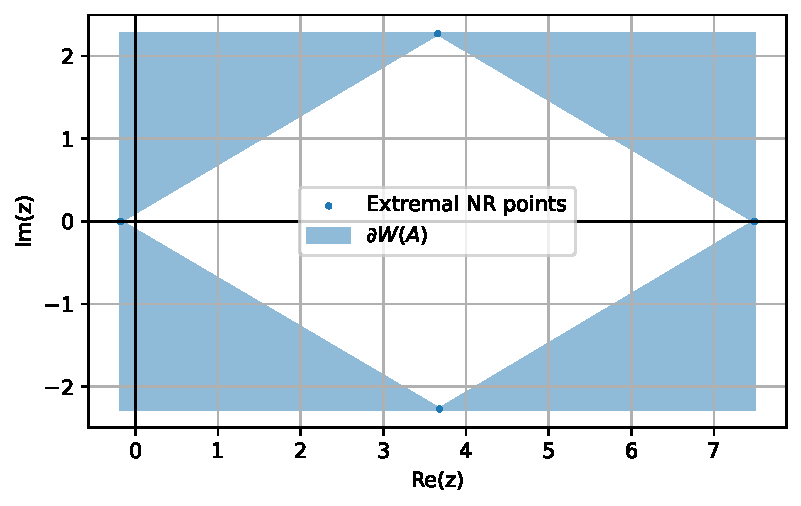
\includegraphics[width=0.3\textwidth]{\dir/img/fine_nr_wc_N4}
% }
% \hfill
\subfloat[$N_{\theta}=8$, $\Delta=0.19$]{
    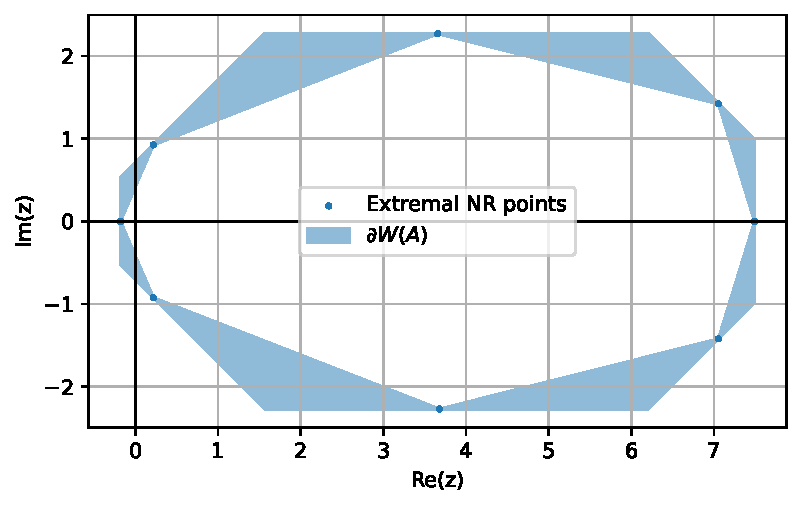
\includegraphics[width=0.3\textwidth]{\dir/img/fine_nr_wc_N8}
}
\hfill
% \subfloat[$N_{\theta}=16$, $\Delta=0.06$]{
%     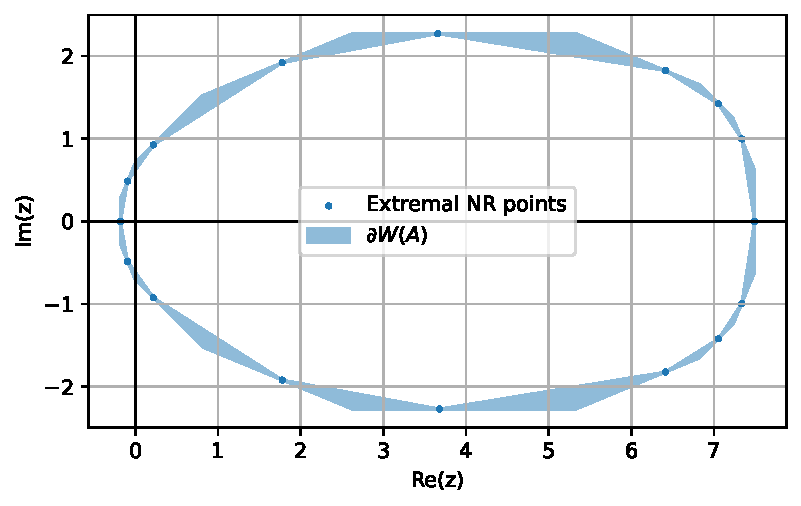
\includegraphics[width=0.3\textwidth]{\dir/img/fine_nr_wc_N16}
% }
% \hfill
\subfloat[$N_{\theta}=32$, $\Delta=0.016$]{
    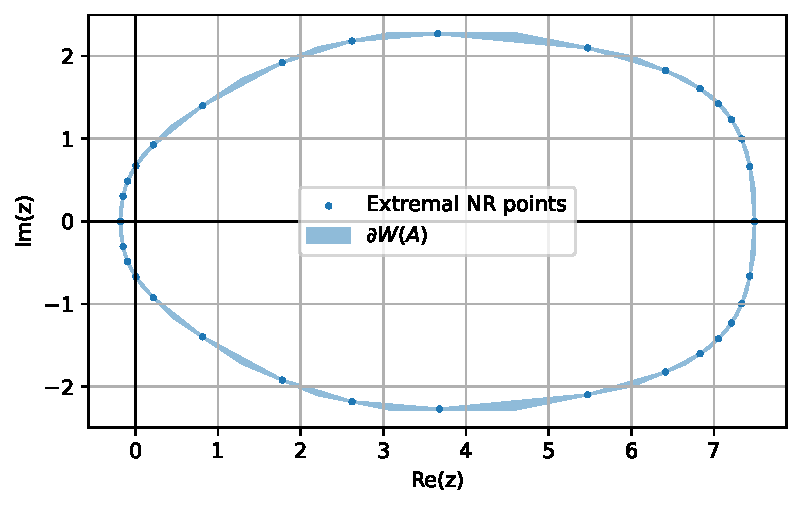
\includegraphics[width=0.3\textwidth]{\dir/img/fine_nr_wc_N32}
}
\hfill
\subfloat[$N_{\theta}=128$, $\Delta=0.001$]{
    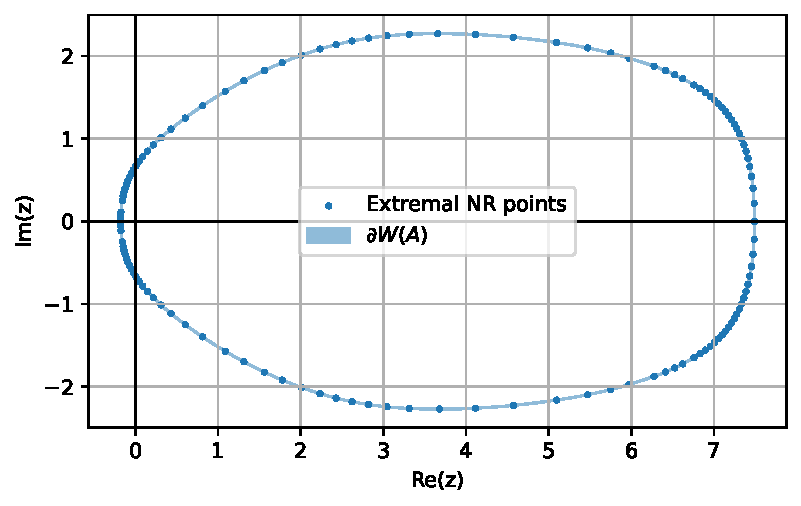
\includegraphics[width=0.3\textwidth]{\dir/img/fine_nr_wc_N128}
}

\caption{
Numerical range boundary using different number of probing angles $N_{\theta}$.
The plots show a clear resolution refinement from left to right.
}
\label{fig:nr:error}
\end{figure}

\section{Spectral hull}
\label{app:C:spectral:hull}

Once the numerical range is determined and we have access to the boundary points $P_{\Theta}$, the spectral hull is straightforward to determine:
The spectral hull is always a subset of the numerical range, \cref{eq:nr:convhull}.
Therefore, the eigenvalues closest to the boundary points of the numerical range $p_{\theta} \in P_{\Theta}$ either lie on the boundary of the spectral hull or outside of it.
It is thus enough to determine the eigenvalues closest to the shifts $p_{\theta} \in P_{\Theta}$, or equivalently the smallest magnitude eigenvalue $\lambda_{\theta}$ of the shifted systems
\begin{equation}
A_{\theta} \psi = \lambda_{\theta} \psi \;,
\quad
\text{with}
\quad
A_{\theta} = A - p_{\theta} \id \;.
\end{equation}
If we do that for $p_{\theta}$ fine enough, we find extremal eigenvalues $\lambda_{\theta}$ of $A$ in all directions probed by the $p_{\theta}$.
The convex hull of the set $\Lambda_{\Theta} = \{ \lambda_{\theta} \}_{\theta}$ gives us a inner approximation of the true spectral hull,
\begin{equation}
\Sigma_{\text{in}} = \convhull{ \Lambda_{\Theta} } \subseteq \convshull{A} \;.
\end{equation}

%Now we can play the same game as for the numerical range with the tangents, since the spectral hull is convex and compact too.
